\documentclass[]{article}
\usepackage{graphicx}

%opening
\title{Assignment 1 CDA}
\author{Tim van Rossum, 4246306\\
	Michiel Doesburg,}

\begin{document}

\maketitle

\section{A visualization of the data}
For the visualization part of this assignment, we first started out by making bar plots of different kinds, but eventually settled  for the scatterplot as seen in figure 1. This scatterplot uses the amount of Eurocent spent per transaction, to allow for better comparisons to be made, as there were five different currencies in the dataset. Exchange rates of April 25, 2018 were used. As can be seen from the scatterplot, there are basically no fraudulent transactions where more than 800 Euro was spent, while there are many benign transactions where more than 800 Euro was spent. Other visualizations we made included the ratio of fraudulent versus non-fraudulent transactions per country and per card issuer. Notable observations were that most nearly all fraudulent transactions come from Mexico and Australia (nearly 90 percent), while these two countries are responsible for very few non-fraudulent transactions. McCredit is responsible for significantly more fraudulent transactions than non-fraudulent. The inverse being true for visadebit, which accounts for roughly 60 percent of benign transactions, yet only 10 percent of fraudulent ones.
\begin{figure}[h!]
	\centering
	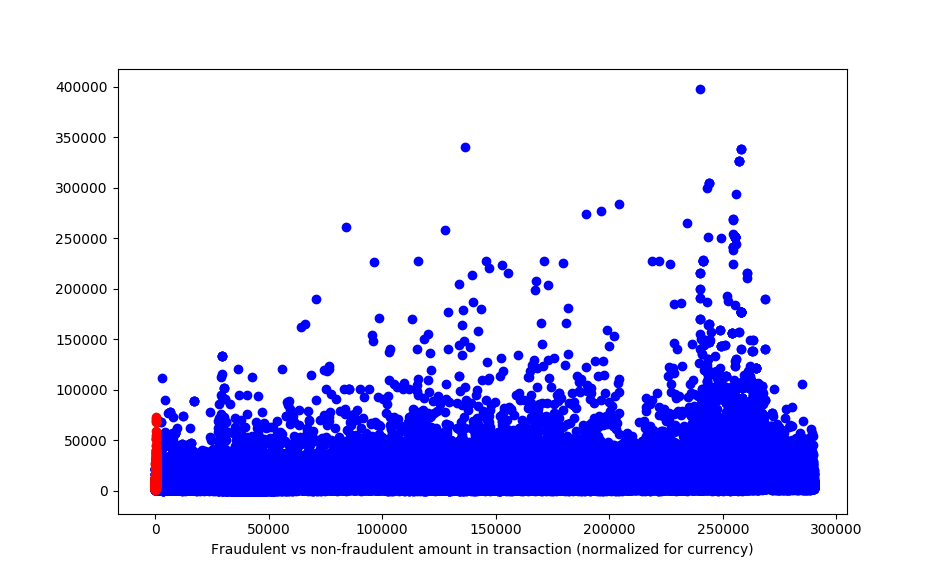
\includegraphics[width=10cm,height=4cm]{Visualizations/AmtFraudvsNonFraud2.png}
	\caption{A scatterplot of the amount of money spent in the sampled transactions. A red dot indicates a fraudulent transaction (these are only at the very left of the plot due to very little fraudulent transactions existing), while a blue dot indicates a benign transaction.}
\end{figure}
\clearpage
\section{Applying SMOTE to the data}
Because we used Python for this assignment with \texttt{scikit-learn}, we used SMOTE as implemented in the package \texttt{imblearn}. The \texttt{fraud\_detection.py} script already preprocessed the data in such a way that applying SMOTE to it was very easy, as the implementation only needed the data and the class labels, and both were already generated by the script. The general steps of preprocessing are: 
\begin{itemize}
	\item Remove data with the "Refused" label (as that is data where we cannot be certain whether or not it is fraudulent)
	\item Remove the ID and booking date of the transaction, as these are not necessary.
	\item Transform the mail identifiers, IP identifiers etc. to simply the number that they use.
\end{itemize}
The classifiers that we used were the random forest classifier, the 5-NN classifier, and the logistic classifier. These were chosen to represent both linear and non-linear classifiers, as well as parametric and non-parametric classifiers (as NN is deemed a non-parametric classifier). The ROC curves are shown in figure 2.
\begin{figure}[h!]
	\centering
	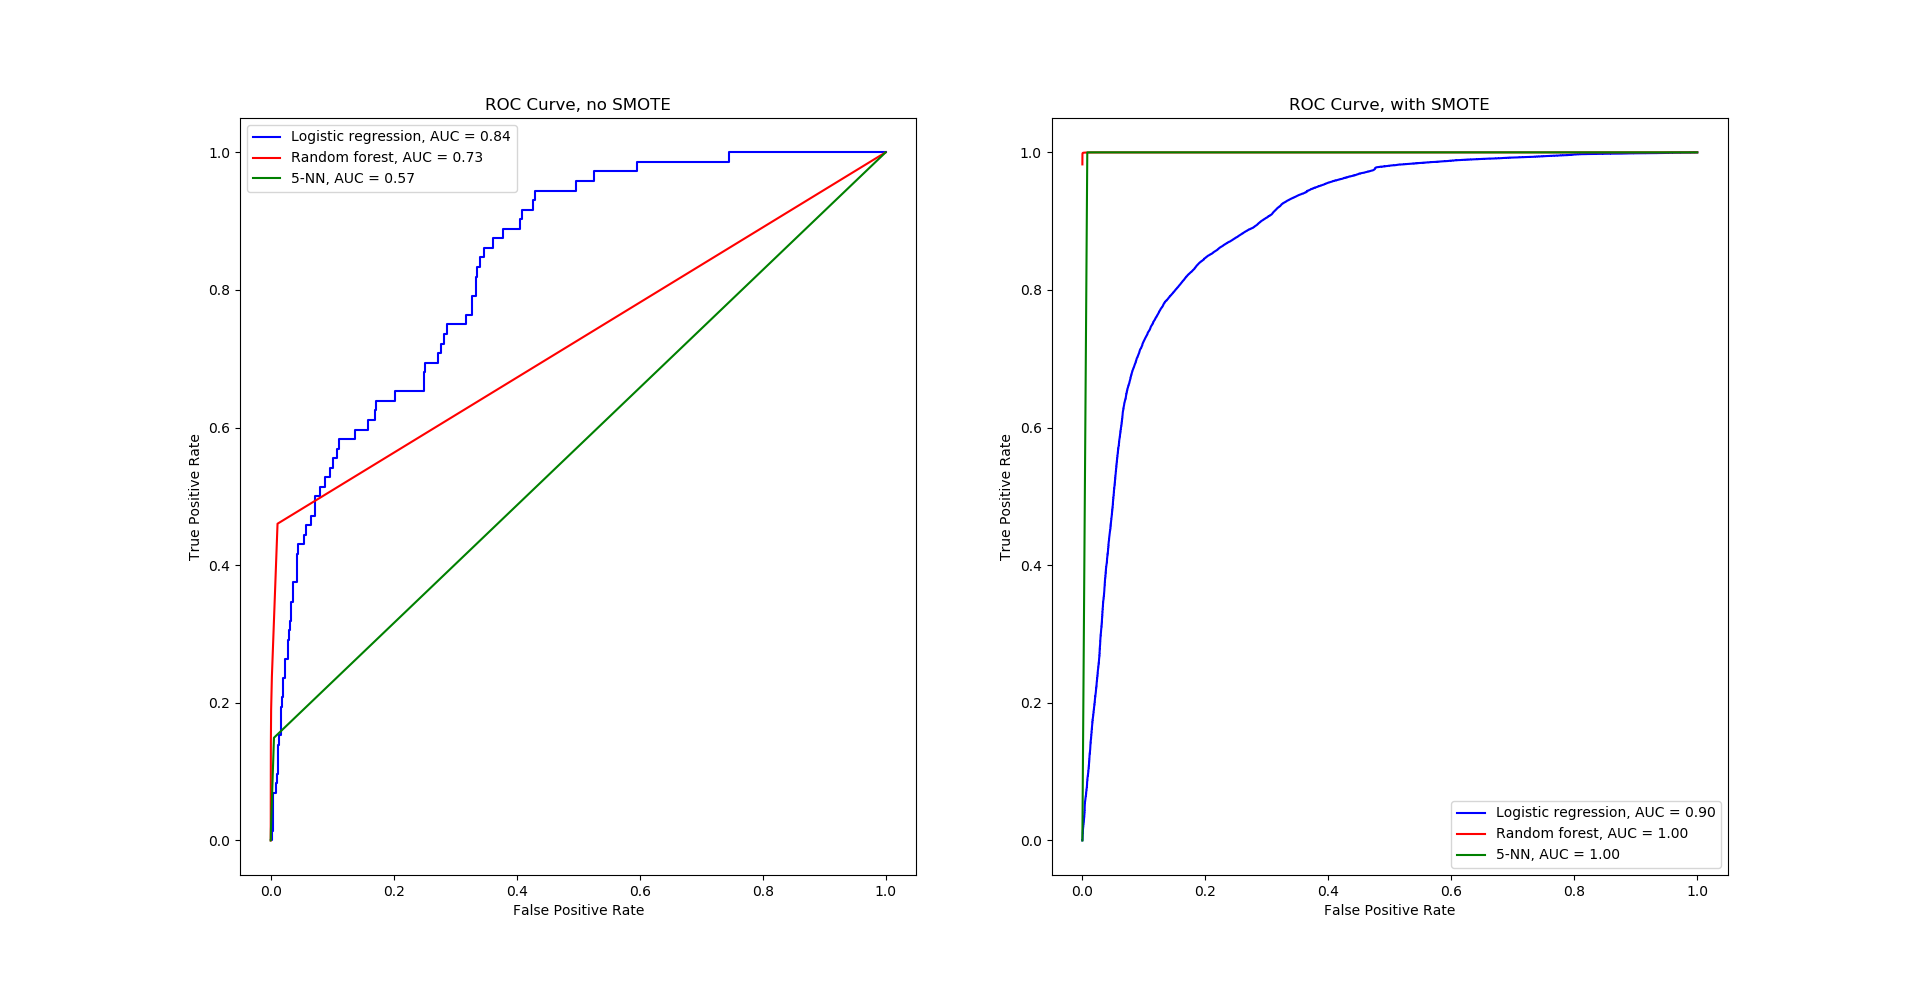
\includegraphics[scale = 0.27]{Visualizations/ROC_curves}
	\caption{The ROC curves, the one on the left does not use SMOTE to oversample training data, and the one on the left does. As can be seen, the area under the curve (AuC) is slightly higher while using SMOTE on training data.}
\end{figure}
\clearpage
\section{The black box and white box classifier}
In this section, we will compare a very simple white box classifier that we wrote with a black box classifier for detecting fraudulent cases in the data. We will also discuss the applicability of both methods in practice.
\subsection{The white box classifier}
For the white box classifier we took a look at several features of the data: issuer country code, transaction variant code, shopper interaction, card verification, CVC response, account code and card issuer identifier. We wrote a small script which, for the fraudulent transactions only, gathered the ranges of values that these features take. A transaction $t$ is labeled as fraudulent if for every feature in the set of features that we use (so, issuer country code, transaction variant code, shopper interaction, card verification, CVC response, account code and card issuer identifier), it has a value that matches the value used in a fraudulent transaction. As this is a white box classifier with simple decision rules, no training will be performed (although one could argue that determining the values of the features selected of the fraudulent cases could technically be seen as learning), and the classifier will classify data directly. Although this is a very simple approach, it seems to work quite well on the test data. This approach produces the following results:

\begin{flushleft}
TP: 155 \newline
FP: 5  \newline
TN: 236686 \newline
FN: 190 \newline
\end{flushleft}

\subsection{The black box classifier}
For the black box classifier, we will be using the random forest classifier, as this classifier tended to perform better, especially on SMOTEd data. It is also a classifier that has been shown to perform better in the papers (TODO ref). In order to train and test this classifier on the data, we will be using ten-fold cross validation, to get a clear picture of how this classifier would perform in practice. We will also be using SMOTE to balance the training data for every round. The performance for this approach is as follows:

\begin{flushleft}
	TP: 23 \newline
	FP: 157  \newline
	TN: 236196 \newline
	FN: 322 \newline
\end{flushleft}
\subsection{Performance and evaluation}
The performance of the black box algorithm is slightly worse than the performance of the white box algorithm, but the white box algorithm is also very simple, and an adversary only has to commit fraud using a different card (that has not been used in a fraudulent transaction before) to prevent being detected. Another way to bypass detection would be to commit fraud in a country that has no recorded fraudulent transactions (which is easier than it seems as around 90\% of all fraudulent transactions happened in Mexico, Australia, the United Kingdom or Sweden). As such, we predict that the white box algorithm will perform very poorly in practice. Contrasting this, the black box algorithm will most likely also perform well in practice, as we do not assume anything about the fraudulent transactions.
\section{Bonus task}
As a way to improve our classifier even further, we tried to convert all the money spent in the transactions to Euros, using the exchange rates, once again, from April 25, 2018. TODO results.

Another thing what we did is not using SMOTE to balance training data while testing the performance of the random forest classifier using ten-fold cross-validation. This resulted in the following performance:
\begin{flushleft}
	TP: 3 \newline
	FP: 5  \newline
	TN: 236348 \newline
	FN: 342 \newline
\end{flushleft}
Interestingly, not using SMOTE results in a far lower false positive rate, which is the main performance metric that we are interested in for developing fraud detection systems. But it should be noted that not using SMOTE causes the random forest classifier to miss a lot more cases as well.
\end{document}
